\section{Random-Access Memory}
\label{sec:ram}

\begin{itemize}[leftmargin=0.6cm]
  \item \textit{A memory unit is a collection of storage cells}, together with associated circuits needed to transfer information into and out of a device.
  \item The time it takes to transfer information to or from any desired random location is always the same -hence the name \textit{random-access memory}, abbreviated RAM.
  \item A memory unit stores binary information in groups of bits called \textbf{\textit{words}}. A \textit{word in memory is a set of bits that move in and out of storage as a unit}.
  \item \textit{A group of 8 bits is called a byte}.
  \item Communication between memory and its environment is achieved through \textit{data input} and \textit{output lines}, \textit{address selection lines}, and \textit{control lines} that specify the direction of transfer. A block diagram of a memory unit is shown in Fig. 2.
\end{itemize}

\begin{figure}[H]
  \centering
  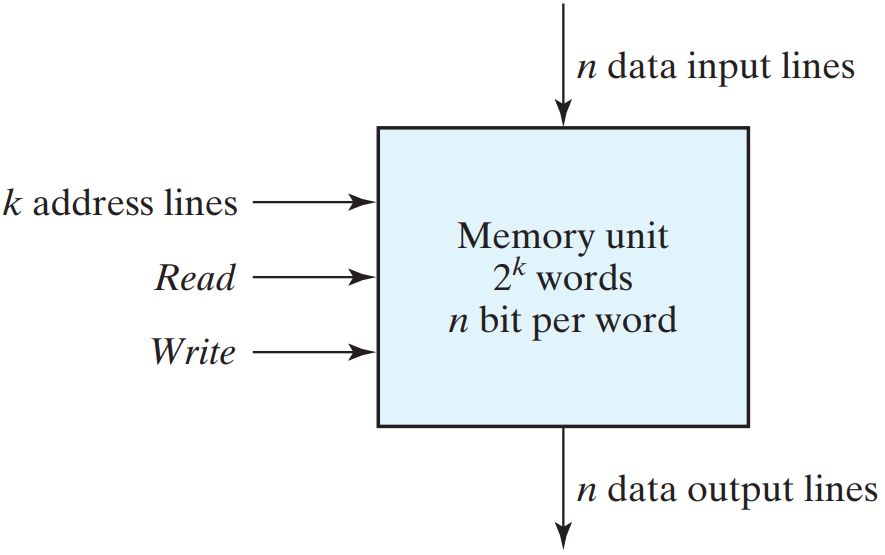
\includegraphics[width=.9\linewidth]{img/fig-7.2.png}
  \caption{Block diagram of a memory unit}
  \label{fig:7.2}
\end{figure}

\begin{itemize}[leftmargin=0.6cm]
  \item The \textit{memory unit is specified by the number of words it contains and the number of bits in each word} ($cell\_size \times word\_size$). The $1K \times 16$ memory of Fig. 3 has 10 bits in the address and 16 bits in each word. Total storage is $2^14$ bits.
\end{itemize}

\begin{figure}[H]
  \centering
  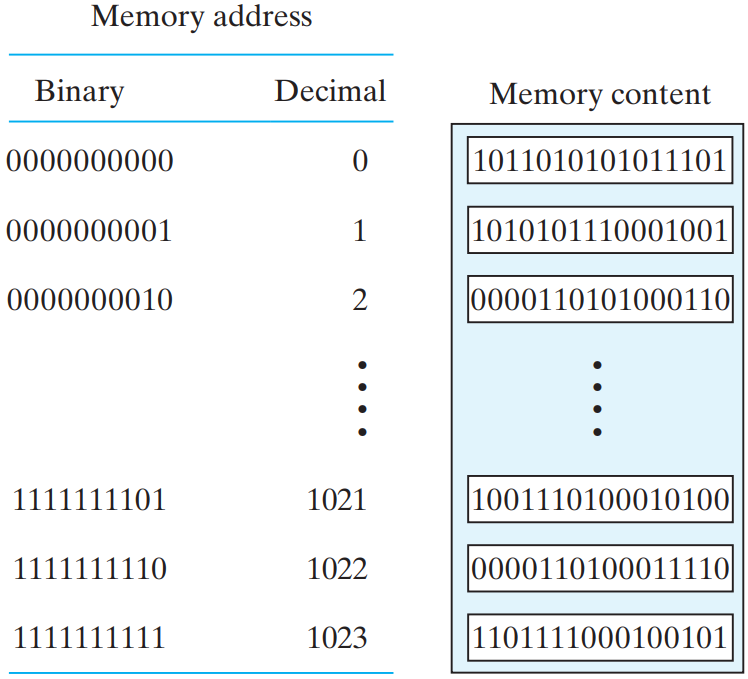
\includegraphics[width=\linewidth]{img/fig-7.3.png}
  \caption{Contents of a $1024 \times 16$ memory}
  \label{fig:7.3}
\end{figure}

\begin{itemize}[leftmargin=0.6cm]
  \item \textit{The number of address bits needed in a memory is dependent on the total number of words that can be stored in the memory and is independent of the number of bits in each word}.
\end{itemize}

\subsection{Write and Read Operations}
\label{subsec:write-read-operations}

\begin{itemize}[leftmargin=0.6cm]
  \item The two operations that RAM can perform are the write and read operations.
  \item The write signal specifies a transfer-in operation and the read signal specifies a transfer-out operation.
  
  \vspace*{\fill}
  \columnbreak

  \item The steps that must be taken for write:
    \begin{enumerate}[leftmargin=0.6cm]
      \item Apply the binary address of the desired word to the address lines.
      \item Apply the data bits that must be stored in memory to the data input lines.
      \item Activate the \textit{write} input.
    \end{enumerate}
  \item The steps that must be taken for read:
    \begin{enumerate}[leftmargin=0.6cm]
      \item Apply the binary address of the desired word to the address lines.
      \item Activate the read input.
    \end{enumerate}
\end{itemize}

The memory operations that result from these control inputs are specified in Table 7.1.
\begin{figure}[H]
  \centering
  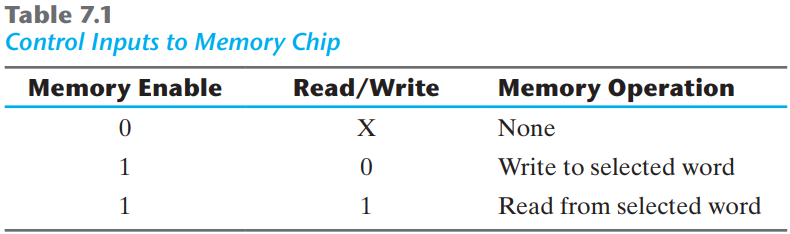
\includegraphics[width=\linewidth]{img/table-7.1.png}
  \label{table:7.1}
\end{figure}

\subsection{Timing Waveforms}
\label{subsec:timing-waveforms}

The operation of the memory unit is controlled by an external device such as a central processing unit (CPU). The CPU is usually synchronized by its own clock. The memory, however, does not employ an internal clock. Instead, its read and write operations are specified by control inputs.
\begin{itemize}
  \item The \textbf{\textit{access time}} of memory is the \textit{time required to select a word and read it}. 
  \item The \textit{\textbf{cycle time}} of memory is the \textit{time required to complete a write operation}.
\end{itemize}

The memory timing shown in Fig. 4 is for a CPU with a 50 MHz clock and a memory with 50 ns maximum cycle time. The write cycle in part (a) shows three 20 ns cycles: $T_1$, $T_2$, and $T_3$. 

\paragraph{Write Operation}

For a write operation, the CPU must provide the address and input data to the memory. This is done at the beginning of $T_1$.

The memory enable and the read/write signals must be activated after the signals in the address lines are stable in order to avoid destroying data in other memory words.

The two control signals must stay active for at least 50 ns. The address and data signals must remain stable for a short time after the control signals are deactivated.

At the completion of the third clock cycle, the memory write operation is completed and the CPU can access the memory again with the next $T_1$ cycle.

\begin{figure}[H]
  \centering
  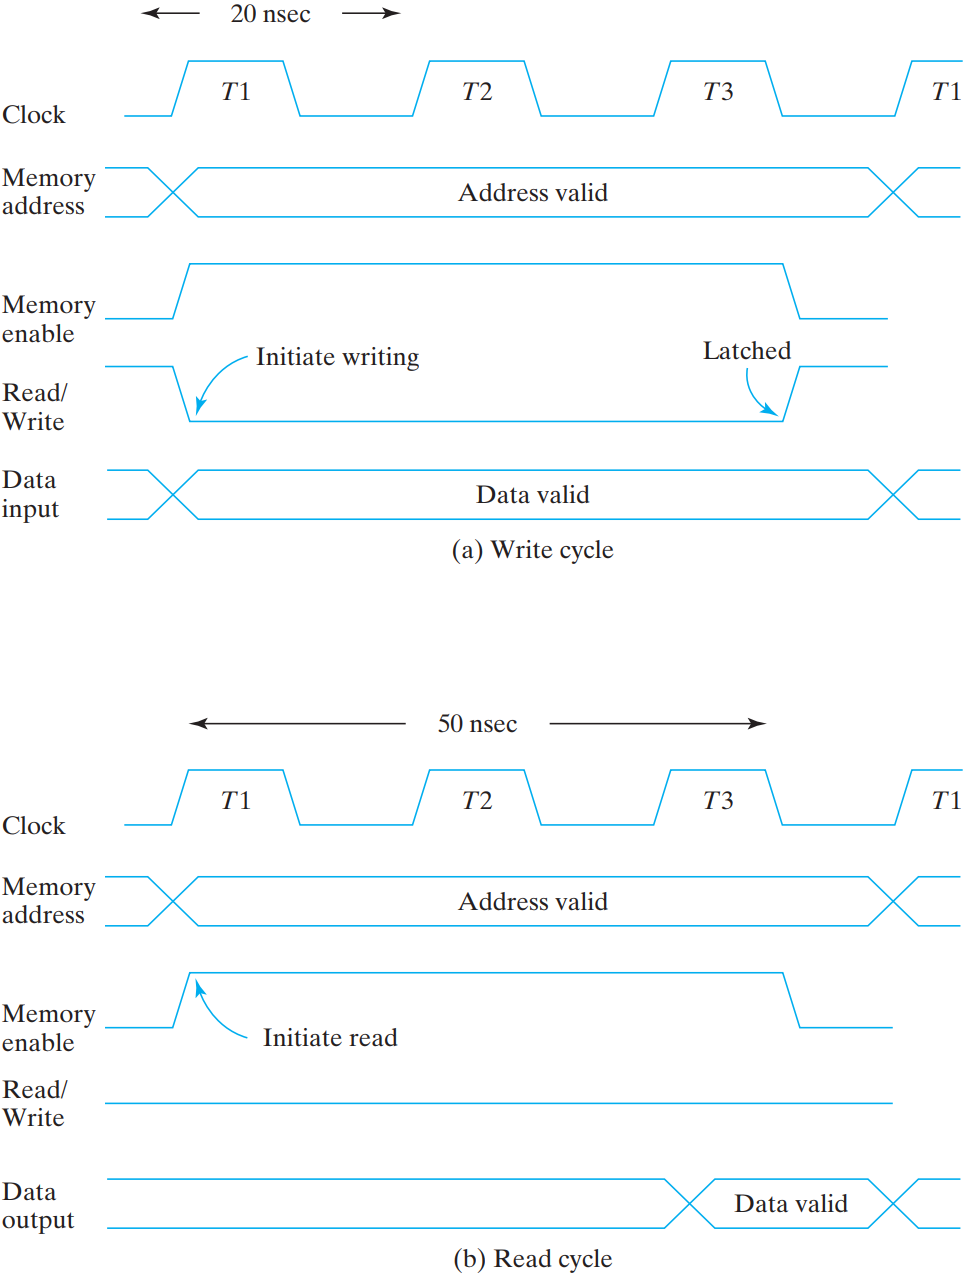
\includegraphics[width=\linewidth]{img/fig-7.4.png}
  \caption{Memory cycle timing waveforms}
  \label{fig:7.4}
\end{figure}

\paragraph{Read Operation}

The read cycle shown in Fig. 4(b) has an address for the memory provided by the CPU.

The memory places the data of the word selected by the address into the output data lines within a 50 ns interval (or less) from the time that the memory enable is activated.

The CPU can transfer the data into one of its internal registers during the negative transition of $T_3$. The next $T_1$ cycle is available for another memory request.

\subsection{Types of Memories}
\label{subsec:types-of-memories}

Integrated circuit RAM units are available in two operating modes: \textit{static} and \textit{dynamic}. 
\begin{itemize}
  \item \textit{\textbf{Static RAM}} (\textit{SRAM}) consists essentially of \textit{internal latches that store the binary information}. The stored information remains valid as long as power is applied to the unit.
  \item \textit{\textbf{Dynamic RAM}} (\textit{DRAM}) \textit{stores the binary information in the form of electric charges on capacitors} provided inside the chip by MOS transistors. The stored charge on the capacitors tends to discharge with time, and the capacitors must be periodically recharged by \textit{refreshing} the dynamic memory.
\end{itemize}

\vspace*{\fill}
\columnbreak

Refreshing is done by cycling through the words every few milliseconds to restore the decaying charge. DRAM offers reduced power consumption and larger storage capacity in a single memory chip. SRAM is easier to use and has shorter read and write cycles.

The reason why latches are used in SRAM is that a latch can be made with only two NAND or two NOR gates, but a flip-flop requires at least twice that much hardware. Also, in general, smaller is faster, cheaper and requires less power.

Dynamic RAMs tend to be physically smaller than static RAMs. So, this means dynamic RAM is cheaper and denser—more bits can be stored in the same physical area. DRAM offers reduced power consumption and larger storage capacity in a single memory chip.
